\documentclass[]{../template/Report}%方括号内写yuxi即生成预习报告\documentclass[yuxi]{../template/Report}
\settemplatedir{../template/}%设置模板路径

\exname{光栅衍射实验} %实验名称
\extable{} %实验桌号
\instructor{王兆英} %指导教师
\class{信工2401} %班级
\name{姚舜瑜} %姓名
\stuid{3240100532} %学号

\nyear{2025} %年
\nmonth{12} %月
\nday{16} %日
\nweekday{二} %星期几，e.g. \nweekday{三}
\daypart{上午}%上午/下午

\redate{} %如有实验补做，补做日期
\resitu{} %情况说明：

\begin{document}
\maketitle%输出封面

\section{预习报告（10分）}

\subsection{实验综述（5分）}

\subsubsection{实验目的}
本实验旨在掌握分光计的调节和使用方法、理解光栅衍射的基本原理的基础上，利用分光计测量透射光栅的光栅常数 $d$ 及角色散率 $D$，同时利用这一原理来测量汞灯谱线的波长 $\lambda$。


\subsubsection{实验原理}
光栅衍射是多缝干涉与单缝衍射的综合效应。如图 \ref{fig:principle} 所示，当波长为 $\lambda$ 的平行光垂直入射到光栅（光栅常数 $d=a+b$）上时，相邻狭缝的衍射光在衍射角为 $\theta$ 的方向上产生光程差 $\Delta = d\sin\theta$。根据干涉加强条件，满足光栅方程的位置出现主极大亮纹：
\begin{equation}
    d \sin \theta = k \lambda \quad (k = 0, \pm 1, \pm 2, \dots)
\end{equation}
实验中利用已知波长的汞灯光源（如绿色谱线 $\lambda=546.1\text{nm}$），测出 $\pm 1$ 级衍射角 $\theta$，即可求出光栅常数 $d$。

此外，光栅的分光能力由角色散率描述。角色散率是衡量光栅作为色散元件，把不同波长的光分开的能力，定义为：
\[
    D = \frac{d\theta}{d\lambda} = \frac{k}{d \cos \theta}
\]
角色散率越大，光栅分辨不同波长光的能力越强。带入先前测得的光栅常数 $d$ 和衍射角 $\theta$，即可计算角色散率 $D$。

根据先前测得的光栅常数 $d$，测量其他谱线的衍射角 $\theta$，亦可计算出对应的波长 $\lambda$。
%--- 图片占位符 1：原理图 ---
\begin{figure}[H]
    \centering
    % 请将 'principle_fig.jpg' 替换为你实际的图片文件名
    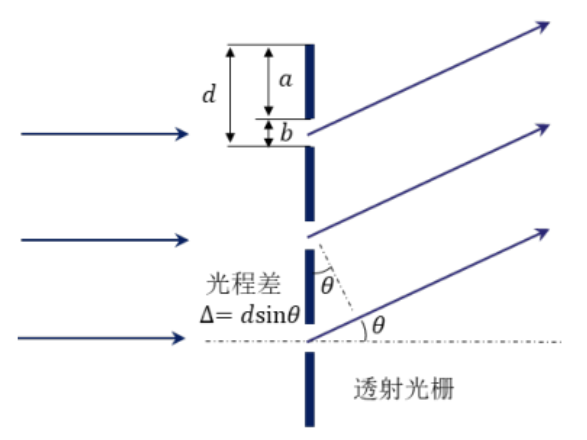
\includegraphics[width=0.4\textwidth]{figures/光栅原理.png} 
    \caption{光栅衍射原理示意图}
    \label{fig:principle}
\end{figure}

\subsubsection{实验方法与步骤}
实验主要分为\textbf{分光计的调节}与\textbf{光栅常数的测量}两部分。实验装置如图 \ref{fig:setup} 所示。

\begin{enumerate}
    \item \textbf{分光计的调节：} 按实验要求调节分光计，使其达到“三垂直”状态（望远镜光轴、平行光管光轴、载物台平面均垂直于仪器主轴）。重点利用\textbf{自准直法}调节望远镜聚焦无穷远，并利用\textbf{各半调节法}校正光轴。调节平行光管发出平行光，并使光栅平面垂直于入射光（利用绿十字像重合）。
    
    \item \textbf{测定光栅常数 $d$ 和角色散率 $D$：} 
    \begin{itemize}
        \item 已知汞灯绿色谱线的波长 $\lambda_{G} = 546.07 \text{ nm}$。
        \item 转动望远镜，测量 $\pm 1$ 级绿色谱线的衍射角。分别读取+1级左右游标盘读数为$\phi_1,\phi_2$，-1级的左右游标盘读数为$\phi'_1,\phi'_2$，计算衍射角 $\theta_G$为：
        \[
        \theta_G = \frac{|\phi_1 -\phi'_1|+| \phi_2 - \phi'_2|}{4}
        \]
        \item 根据光栅方程 $d \sin \theta_G = 1 \cdot \lambda_G$ 计算光栅常数 $d$ 及其不确定度。
        \item 根据公式 $D = \frac{1}{d \cos \theta_G}$ 计算角色散率 $D$ 及其不确定度。
    \end{itemize}
    
    \item \textbf{测定其他谱线的波长：}
    \begin{itemize}
        \item 观察并测量汞灯光谱中\textbf{紫色、蓝色、黄色}谱线的 $\pm 1$ 级衍射角。
        \item 记录各谱线左右游标盘的读数，计算对应的衍射角 $\theta$。
        \item 利用已测得的光栅常数 $d$，通过光栅方程 $\lambda = d \sin \theta$ 计算各谱线的波长。
    \end{itemize}
\end{enumerate}

\begin{figure}[H]
    \centering
    \begin{minipage}[b]{0.48\textwidth}
        \centering
        % 设置固定高度以保证并排对齐
        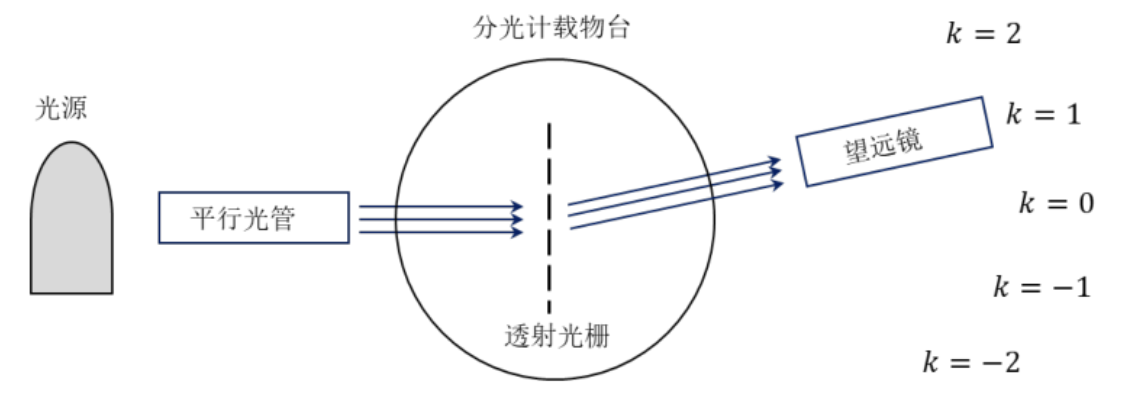
\includegraphics[height=3.7cm]{figures/分光计载物台.png}
        \caption{分光计测量衍射角结构示意图}
        \label{fig:setup}
    \end{minipage}
    \hfill
    \begin{minipage}[b]{0.48\textwidth}
        \centering
        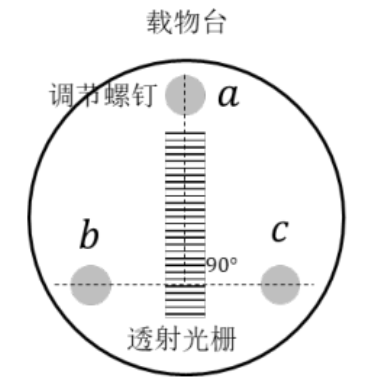
\includegraphics[height=3.7cm]{figures/载物台示意图.png}
        \caption{透射光栅摆放位置示意图}
        \label{fig:grating_pos}
    \end{minipage}
\end{figure}
\subsubsection{进阶实验}
\begin{enumerate}
    \item \textbf{绿光二级光谱测量：} 测量绿色谱线二级光谱的衍射角，计算光栅常数 $d$ 和角色散率 $D$，并与一级光谱结果比较。
    \item \textbf{分辨黄色双线：} 选择合适级次分辨汞灯黄色双线，测量衍射角变化 $\Delta \theta$ 并计算 $\Delta \lambda$，比较两种角色散率计算公式（$D = \frac{\Delta \theta}{\Delta \lambda}$ 与 $D = \frac{k}{d \cos \theta}$）的结果。
    \item \textbf{旋转光栅实验：} 旋转光栅改变入射角约 $10^\circ$，测量绿光衍射角变化，比较 $\pm 1$ 级衍射角差异并分析原因。
\end{enumerate}

\subsection{实验重点（3分）}

\begin{enumerate}
    \item \textbf{分光计调节：} 掌握望远镜聚焦无穷远（消除视差）及光轴垂直于仪器主轴（各半调节法）的操作。
    \item \textbf{数据读取：} 熟悉双游标读数方法以消除偏心差，准确读取角度值。
    \item \textbf{光栅调节：} 调节光栅平面垂直于入射光，确保衍射光谱分布对称。
\end{enumerate}

\subsection{实验难点（2分）}
\begin{enumerate}
    \item \textbf{消除视差：} 望远镜观察时需精确调节物镜和分划板位置，确保像落在分划板平面上，避免视差引入读数误差。
    \item \textbf{读数精度：} 双游标读数要求操作熟练，需多次测量取平均以减小随机误差。
    \item \textbf{光栅调节：} 光栅平面需严格垂直于入射光，调节不当会导致衍射角偏移，影响测量结果。
\end{enumerate}

\begin{fullreportonly}
\section{原始数据（20分）}
\begin{figure}[H]
  \centering
  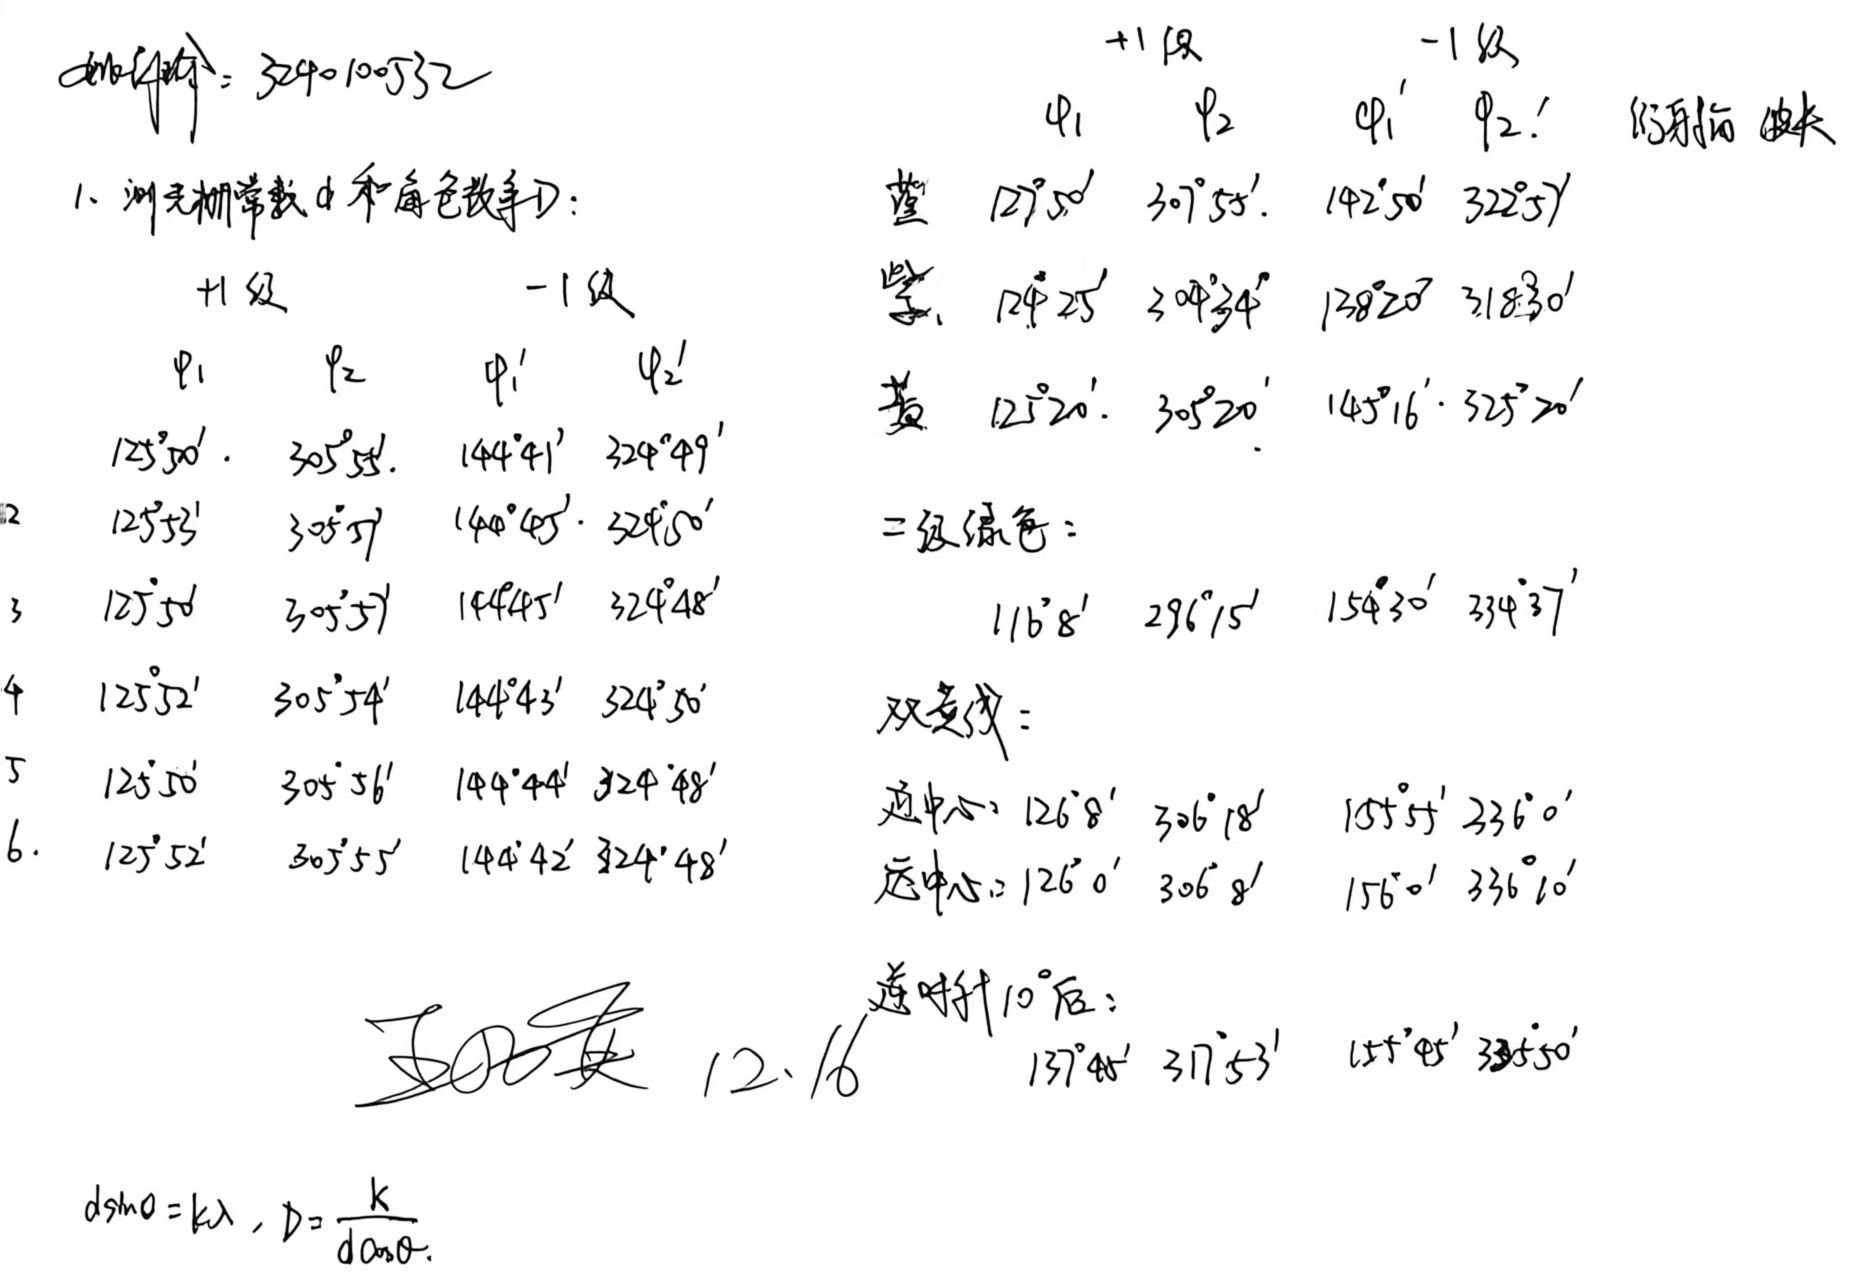
\includegraphics[width=0.8\textwidth]{figures/实验数据.jpg}
  \caption{实验数据照片}
\end{figure}

\section{结果与分析（60分）}

\subsection{数据处理与计算（30分）}

\subsubsection{测量光栅常数 $d$ 和角色散率 $D$（绿光 $k=1$）}
已知汞灯绿色谱线波长 $\lambda_G = 546.07 \text{ nm}$。

\begin{table}[H]
    \centering
    \caption{绿光（$k=1$）衍射角测量数据}
    \begin{tabular}{ccccccc}
        \toprule
        \multirow{2}{*}{序号} & \multicolumn{2}{c}{+1级读数} & \multicolumn{2}{c}{-1级读数} & \multirow{2}{*}{$2\theta$} & \multirow{2}{*}{$\theta$} \\
        \cmidrule(lr){2-3} \cmidrule(lr){4-5}
         & $\varphi_1$ & $\varphi_2$ & $\varphi_1'$ & $\varphi_2'$ & & \\
        \midrule
        1 & $125^\circ 50'$ & $305^\circ 55'$ & $144^\circ 41'$ & $324^\circ 49'$ & $18^\circ 52'$ & $9^\circ 26'$ \\
        2 & $125^\circ 53'$ & $305^\circ 57'$ & $144^\circ 45'$ & $324^\circ 50'$ & $18^\circ 52'$ & $9^\circ 26'$ \\
        3 & $125^\circ 50'$ & $305^\circ 57'$ & $144^\circ 45'$ & $324^\circ 48'$ & $18^\circ 53'$ & $9^\circ 27'$ \\
        4 & $125^\circ 52'$ & $305^\circ 54'$ & $144^\circ 43'$ & $324^\circ 50'$ & $18^\circ 54'$ & $9^\circ 27'$ \\
        5 & $125^\circ 50'$ & $305^\circ 56'$ & $144^\circ 44'$ & $324^\circ 48'$ & $18^\circ 53'$ & $9^\circ 27'$ \\
        6 & $125^\circ 52'$ & $305^\circ 55'$ & $144^\circ 42'$ & $324^\circ 48'$ & $18^\circ 52'$ & $9^\circ 26'$ \\
        \bottomrule
    \end{tabular}
\end{table}

\textbf{计算结果：}
\begin{itemize}
    \item 平均衍射角：$\bar{\theta}_G =\frac{9^\circ 26'\times 3 + 9^\circ 27' \times 3}{6} \approx 9^\circ 26' = 9.4333^\circ$
    \item 光栅常数：$d = \frac{\lambda}{\sin \bar{\theta}_G} = \frac{546.07}{\sin(9.4333^\circ)} = 3332.0 \text{ nm}$
    \item 角色散率：$D = \frac{1}{d \cos \bar{\theta}_G} = \frac{1}{3332.0 \times \cos(9.4333^\circ)} = 3.042 \times 10^{-4} \text{ rad/nm}$
\end{itemize}

\subsubsection{测量其他谱线波长}
利用计算得到的光栅常数 $d = 3332.0 \text{ nm}$，根据 $\lambda = d \sin \theta$ 计算各谱线波长。

\begin{table}[H]
    \centering
    \caption{各色光衍射角及波长计算结果}
    \begin{tabular}{ccccccc}
        \toprule
        \multirow{2}{*}{谱线} & \multicolumn{2}{c}{+1级} & \multicolumn{2}{c}{-1级} & \multirow{2}{*}{$\theta$} & \multirow{2}{*}{计算波长 $\lambda$ (nm)} \\
        \cmidrule(lr){2-3} \cmidrule(lr){4-5}
         & $\varphi_1$ & $\varphi_2$ & $\varphi_1'$ & $\varphi_2'$ & & \\
        \midrule
        紫光 & $124^\circ 25'$ & $304^\circ 34'$ & $138^\circ 20'$ & $318^\circ 30'$ & $6^\circ 58'$ & $404.2$ \\
        蓝光 & $127^\circ 50'$ & $307^\circ 55'$ & $142^\circ 50'$ & $322^\circ 57'$ & $7^\circ 30'$ & $434.9$ \\
        黄光 & $125^\circ 20'$ & $305^\circ 20'$ & $145^\circ 16'$ & $325^\circ 20'$ & $9^\circ 59'$ & $577.6$ \\
        \bottomrule
    \end{tabular}
\end{table}


\subsubsection{进阶实验数据处理}

\paragraph{(1) 绿光二级光谱测量 ($k=2$)} \mbox{}
\begin{table}[H]
    \centering
    \caption{二级谱线测量数据}
    \begin{tabular}{ccccc}
        \toprule
        \multirow{2}{*}{项目} & \multicolumn{2}{c}{+1级} & \multicolumn{2}{c}{-1级} \\
        \cmidrule(lr){2-3} \cmidrule(lr){4-5}
         & $\varphi_1$ & $\varphi_2$ & $\varphi_1'$ & $\varphi_2'$ \\
        \midrule
        二级绿色 & $116^\circ 08'$ & $296^\circ 15'$ & $154^\circ 30'$ & $334^\circ 37'$ \\
        \bottomrule
    \end{tabular}
\end{table}

\textbf{数据处理：}
\begin{itemize}
    \item \textbf{二级衍射角 $\theta_2$：}
    \[
    \theta_2 = \frac{|116^\circ 08' - 154^\circ 30'| + |296^\circ 15' - 334^\circ 37'|}{4} = \frac{38^\circ 22' + 38^\circ 22'}{4} = 19^\circ 11' = 19.183^\circ
    \]
    \item \textbf{光栅常数 $d'$：}
    \[
    d' = \frac{2\lambda}{\sin \theta_2} = \frac{2 \times 546.07}{\sin(19.183^\circ)} = 3323.6 \text{ nm}
    \]
    与一级光谱测得的 $d=3332.0 \text{ nm}$ 相比，相对差异为 $0.25\%$，吻合良好。
    \item \textbf{角色散率 $D_2$：}
    \[
    D_2 = \frac{2}{d' \cos \theta_2} = \frac{2}{3323.6 \times \cos(19.183^\circ)} = 6.37 \times 10^{-4} \text{ rad/nm}
    \]
    \textbf{结论：} 二级光谱的角色散率约为一级光谱 ($3.04 \times 10^{-4}$) 的 2 倍，验证了 $D \propto k$。
\end{itemize}

\paragraph{(2) 分辨黄色双线} \mbox{}
\begin{table}[H]
    \centering
    \caption{黄色双线测量数据}
    \begin{tabular}{ccccc}
        \toprule
        \multirow{2}{*}{项目} & \multicolumn{2}{c}{+1级} & \multicolumn{2}{c}{-1级} \\
        \cmidrule(lr){2-3} \cmidrule(lr){4-5}
         & $\varphi_1$ & $\varphi_2$ & $\varphi_1'$ & $\varphi_2'$ \\
        \midrule
        双黄线 (近中心) & $126^\circ 08'$ & $306^\circ 18'$ & $155^\circ 55'$ & $336^\circ 00'$ \\
        双黄线 (远中心) & $126^\circ 00'$ & $306^\circ 08'$ & $156^\circ 00'$ & $336^\circ 10'$ \\
        \bottomrule
    \end{tabular}
\end{table}

\textbf{数据处理：}
\begin{itemize}
    \item \textbf{衍射角计算：}
    \begin{itemize}
        \item 线1 (近)：$\theta_{Y1} = (|126^\circ 08' - 155^\circ 55'| + |306^\circ 18' - 336^\circ 00'|)/4 \approx 14^\circ 52'$
        \item 线2 (远)：$\theta_{Y2} = (|126^\circ 00' - 156^\circ 00'| + |306^\circ 08' - 336^\circ 10'|)/4 \approx 15^\circ 00'$
    \end{itemize}
    \item \textbf{微小量计算：}
    \begin{itemize}
        \item 角度差：$\Delta \theta = \theta_{Y2} - \theta_{Y1} = 8' = 0.1333^\circ = 2.33 \times 10^{-3} \text{ rad}$
        \item 波长差 (取 $d=3332.0 \text{ nm}$):
        \[
        \lambda_1 = d \sin \theta_{Y1} = 854.9 \text{ nm}, \quad \lambda_2 = d \sin \theta_{Y2} = 862.4 \text{ nm}
        \]
        \[
        \Delta \lambda = 7.5 \text{ nm}
        \]
    \end{itemize}
    \item \textbf{角色散率比较：}
    \begin{itemize}
        \item 实验值：$D_{exp} = \frac{\Delta \theta}{\Delta \lambda} = \frac{2.33 \times 10^{-3}}{7.5} = 3.11 \times 10^{-4} \text{ rad/nm}$
        \item 理论值：$D_{theo} = \frac{k}{d \cos \bar{\theta}} \approx \frac{1}{3332.0 \times \cos(14.9^\circ)} = 3.11 \times 10^{-4} \text{ rad/nm}$
        \item 两者非常接近，验证了角色散率公式的正确性。
    \end{itemize}
\end{itemize}

\paragraph{(3) 旋转光栅实验} \mbox{}
\begin{table}[H]
    \centering
    \caption{偏转测量数据（逆时针 $10^\circ$）}
    \begin{tabular}{ccccc}
        \toprule
        \multirow{2}{*}{条件} & \multicolumn{2}{c}{读数 1 (左侧谱线)} & \multicolumn{2}{c}{读数 2 (右侧谱线)} \\
        \cmidrule(lr){2-3} \cmidrule(lr){4-5}
         & $\varphi_1$ & $\varphi_2$ & $\varphi_1'$ & $\varphi_2'$ \\
        \midrule
        逆时针 $10^\circ$ & $137^\circ 45'$ & $317^\circ 53'$ & $155^\circ 45'$ & $335^\circ 50'$ \\
        \bottomrule
    \end{tabular}
\end{table}

\textbf{数据处理与分析：}

通过实验数据可以计算出旋转光栅后左右谱线的衍射角，结果为：
\[
    \theta = \frac{|137^\circ 45' - 155^\circ 45'| + |317^\circ 53' - 335^\circ 50'|}{4} = \frac{18^\circ 0' + 17^\circ 57'}{4} = 8^\circ 59' = 8.983^\circ
\]

与未旋转时的 $\theta_G = 9^\circ 26'$ 相比，可以看出，旋转光栅导致衍射角发生了变化。

这说明入射角的改变使得 $\pm 1$ 级衍射角不再对称，符合光栅方程中入射角的影响。具体来说，逆时针旋转光栅相当于增加了入射角 $i$，根据调整后的光栅方程：
\[
d(\sin \theta_k - \sin i) = k\lambda
\]
正级和负级的衍射角将不再相等，从而导致测量结果的差异。

如若使用斜入射的光栅方程进行计算d和D（推导过程见思考题），则可以得到：
\[
    d_{\text{旋转}} = \frac{\lambda}{\sin \theta-\sin i} \quad , \quad D_{\text{旋转}} = \frac{1}{d_{\text{旋转}} \cos \theta}
\]
通过计算得到：
\[
    d_{\text{旋转}} \approx 3325.5 \text{ nm} \quad , \quad D_{\text{旋转}} \approx 3.05 \times 10^{-4} \text{ rad/nm}
\]
与未旋转时的结果相比，光栅常数和角色散率均未发生显著变化，说明光栅本身性质不变，但衍射角受入射角影响。


\subsection{误差分析（20分）}

\subsubsection{衍射角 $\theta$ 的不确定度}
\begin{itemize}
    \item \textbf{A类不确定度}（标准差）：
    \[
    u_A(\theta) = \sqrt{\frac{\sum (\theta_i - \bar{\theta})^2}{n(n-1)}} \approx 10'' \approx 4.85 \times 10^{-5} \text{ rad}
    \]
    \item \textbf{B类不确定度}（仪器误差 $\Delta_{inst} = 1'$）：
    \[
    u_B(\theta) = \frac{\Delta_{inst}}{\sqrt{3}} = \frac{60''}{\sqrt{3}} \approx 35'' \approx 1.70 \times 10^{-4} \text{ rad}
    \]
    \item \textbf{合成不确定度}：
    \[
    u(\theta) = \sqrt{u_A^2 + u_B^2} \approx 36'' \approx 1.75 \times 10^{-4} \text{ rad}
    \]
\end{itemize}

所以衍射角的最终结果为：
\begin{align*}
\overline{\theta} &= 9.4333^\circ \pm  1.75 \times 10^{-4} \text{ rad}  \\
 &= 0.16464 \text{ rad} \pm 1.75 \times 10^{-4} \text{ rad} \\
 &= (1.6464 \pm 0.0018)\times 10^{-1} \text{ rad} \quad (k=1)
\end{align*}
\subsubsection{光栅常数 $d$ 的不确定度}
根据 $d = \lambda / \sin \theta$，不确定度传递公式为：
\[
\frac{u(d)}{d} = |\cot \theta| \cdot u(\theta)
\]
代入数据：
\[
u(d) = 3332.0 \times \cot(9.4333^\circ) \times 1.75 \times 10^{-4} \approx 3.5 \text{ nm}
\]
最终结果：
\[
d = (3332 \pm 4) \text{ nm} \quad (k=1)
\]

\subsubsection{角色散率 $D$ 的不确定度}
根据 $D = \frac{\tan \theta}{\lambda}$，不确定度传递公式为：
\[
u(D) = \frac{\sec^2 \theta}{\lambda} u(\theta) = D \frac{1}{\sin\theta \cos\theta} u(\theta)
\]
代入数据：
\[
u(D) = 3.042 \times 10^{-4} \times \frac{1}{\sin(9.4333^\circ)\cos(9.4333^\circ)} \times 1.75 \times 10^{-4} \approx 0.003 \times 10^{-4} \text{ rad/nm}
\]
最终结果：
\[
D = (3.042 \pm 0.003) \times 10^{-4} \text{ rad/nm}
\]


\subsubsection{波长测量的相对误差}
\begin{itemize}
    \item \textbf{紫光} ($\lambda_{std} = 404.7 \text{ nm}$): $E = \frac{|404.2 - 404.7|}{404.7} \times 100\% = 0.12\%$
    \item \textbf{蓝光} ($\lambda_{std} = 435.8 \text{ nm}$): $E = \frac{|434.9 - 435.8|}{435.8} \times 100\% = 0.21\%$
    \item \textbf{黄光} ($\lambda_{std} = 579.0 \text{ nm}$): $E = \frac{|577.6 - 579.0|}{579.0} \times 100\% = 0.24\%$
\end{itemize}

可以看出，测量波长与标准值的相对误差均小于0.3\%，说明实验结果较为准确，误差在可接受范围内。
\subsection{实验探讨（10分）}
本次实验通过分光计测量光栅衍射现象，验证了光栅方程和角色散率的理论。在理论层面上，我对光栅衍射的理解更加深入了，知道光栅常数和衍射角的关系，以及如何通过测量衍射角来计算波长。
在实验层面上，我掌握了分光计的调节方法，并学会了如何寻找和测量不同级次的衍射谱线。并且，我也对数据处理和误差分析有了更深的理解，能够计算不确定度并评估实验结果的准确性。

\section{思考题（10分）}

\subsection{调节光栅时如发现谱线倾斜，可能是什么原因?应如何调整?}

\paragraph{答：}可能是因为光栅刻痕线与分光计主轴不平行。调整方法是调节载物台下的调平螺丝，改变光栅平面的倾角；或者是调整平行光管的竖直窄缝角度，使之和光栅平行。直到两侧谱线等高且不倾斜。

\subsection{平行光管狭缝太宽或太窄是会出现什么现象?为什么?}

\paragraph{答：}太宽太窄都会影响光栅衍射谱线的质量：\mbox{}

狭缝太宽会导致谱线变宽，分辨率降低，相邻谱线可能重叠无法分辨；

狭缝太窄会导致透光量不足，谱线亮度过暗，难以观察和测量。

\subsection{试推导平行光斜入射时的光栅方程，解释提升内容3的现象。}

\paragraph{答：}设入射角为 $i$，衍射角为 $\theta_k$（均相对于光栅法线）。此时光路图如图所示：\mbox{}

\begin{figure}[H]
    \centering
    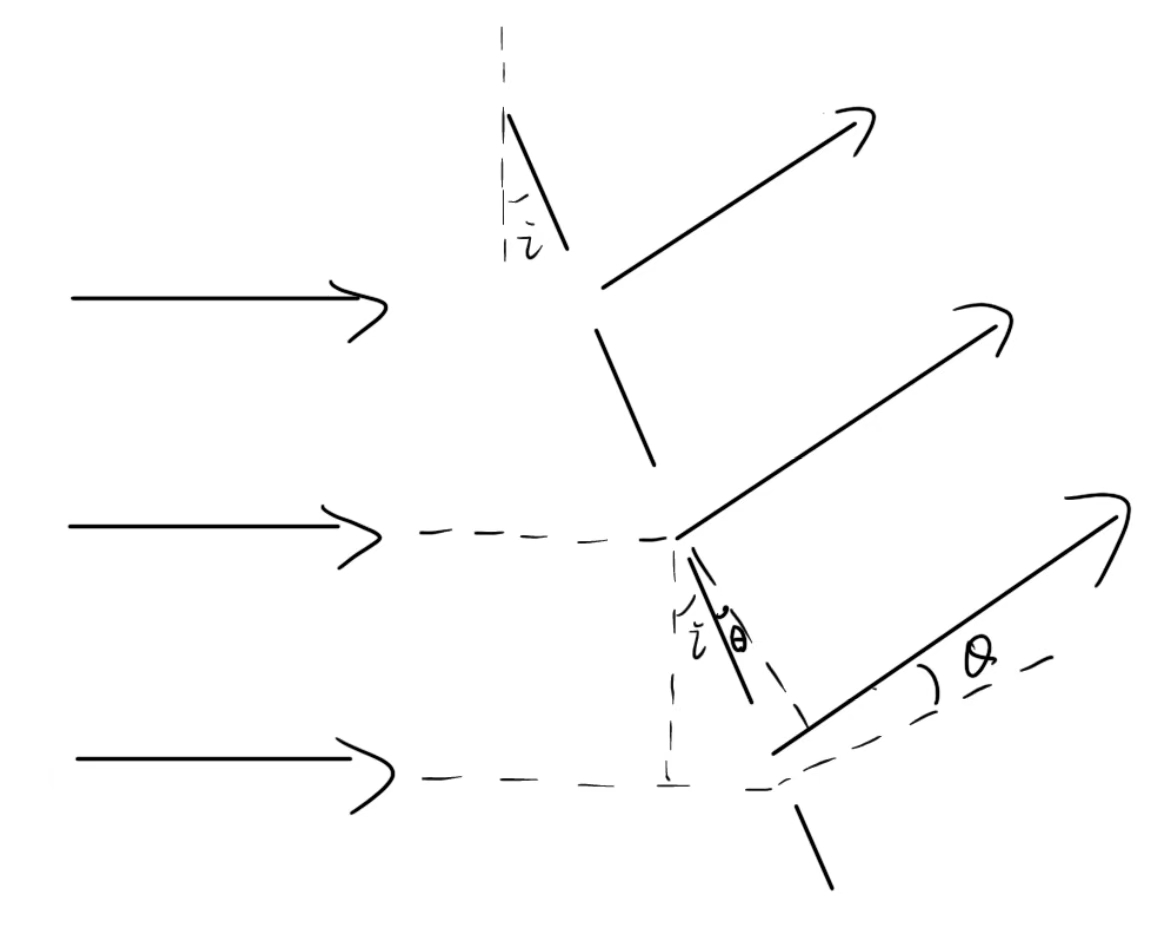
\includegraphics[width=0.4\textwidth]{figures/斜入射.jpg} 
    \caption{平行光斜入射光栅示意图}
    \label{fig:oblique_incidence}
\end{figure}
可以看出相邻两束光线的光程差由两部分组成：入射部分 $AB$ 和衍射部分 $CD$。根据几何关系，有：
\[AB = d \sin i \quad , \quad CD = d \sin \theta_k
\]

因此则相邻狭缝的光程差为：
\[\Delta = d(\sin \theta_k - \sin i)
\]

根据干涉加强条件，主极大亮纹出现时光程差满足：
\[d(\sin \theta_k - \sin i) = k \lambda \quad (k = 0, \pm 1, \pm 2, \dots)
\]

这就是平行光斜入射时的光栅方程。
\subsection{用本实验装置可以分辨钠灯黄色双线(589.0nm与 589.6nm)吗?如果
可以，试给出方案。如果不行，试提出改进方案。}

\paragraph{答：}根据本实验的实际结果显示，可以清晰地看见汞灯黄色双线，说明实验装置的分辨能力足以分辨钠灯黄色双线（波长差仅为0.6nm）。而如若遇到无法分辨的情况，可以调节狭缝至尽可能窄，仔细观察黄光光谱，应能看到两条靠得很近的黄线。若看不清，还可尝试使用二级光谱来观察，间隔缝隙会更大。

\end{fullreportonly}
\insertnotes
\end{document}